\documentclass{beamer}

\begin{document}

\begin{frame}
\frametitle{Método de diferencias divididas}

El método de diferencias divididas se utiliza para aproximar una función $f(x)$ en un conjunto de puntos $x_0$, $x_1$, ..., $x_n$. La idea básica detrás del método es que podemos construir un polinomio interpolante que pase por los puntos dados utilizando las diferencias divididas de la función $f(x)$. 

\[
P_n(x)=a_0 + a_1(x-x_0) +a_2(x-x_0) (x-x_1) + . . . +a_n(x-x_0)...(x-x_n)
\]
\end{frame}




\begin{frame}
\frametitle{Método de diferencias divididas (continuación)}

Las diferencias divididas se definen como:
$$
f[x_0] = f(x_0)
$$

$$
f[x_1,x_0] = \frac{f[x_1] - f[x_0]}{x_1 - x_0}
$$

$$
f[x_2,x_1,x_0] = \frac{f[x_2,x_1] - f[x_1,x_0]}{x_2 - x_0}
$$

$$
...
$$

$$
f[x_n,...,x_0] = \frac{f[x_n,...,x_1] - f[x_{n-1},...,x_0]}{x_n - x_0}
$$

\end{frame}



\begin{frame}{Algoritmo Diferencias divididas}
 \begin{figure}
    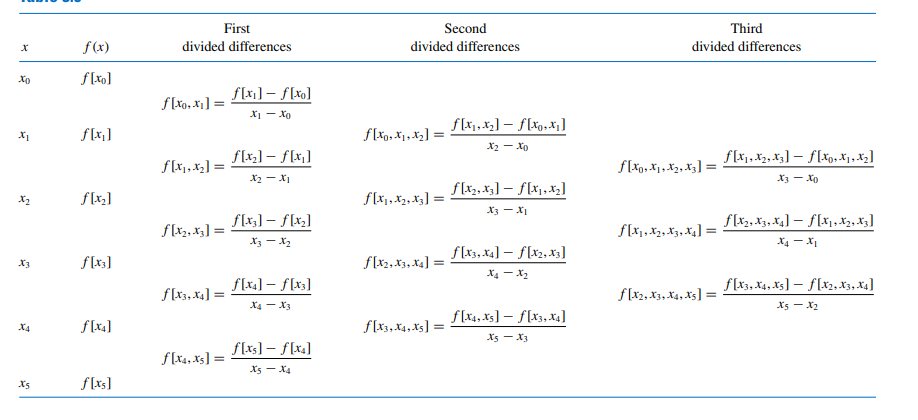
\includegraphics[width=0.9\textwidth]{esquemadiferenciasDivividas.png}
    \caption{Diferencias divididas, Burden, R. L., Faires, J. D., & Burden, A. M. (2017). Análisis numérico (10a. ed.).  } 
\end{figure} 
\end{frame}



\begin{frame}{Algoritmo Diferencias divididas}
 \begin{figure}
    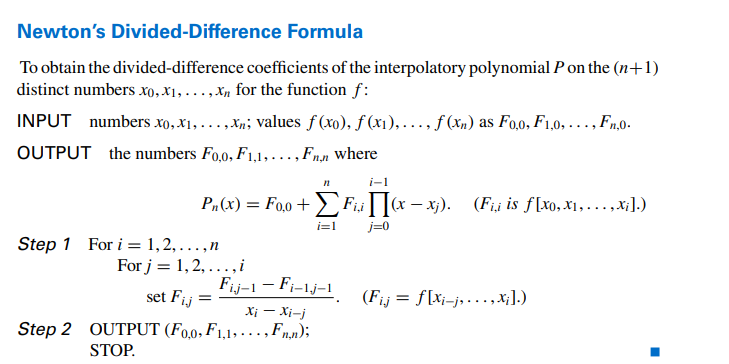
\includegraphics[width=0.9\textwidth]{dividdas.png}
    \caption{Diferencias divididas, Burden, R. L., Faires, J. D., & Burden, A. M. (2017). Análisis numérico (10a. ed.).  } 
\end{figure} 
\end{frame}



\begin{frame}
\frametitle{Método de diferencias divididas (Ejemplo)}

Una vez que se han calculado las diferencias divididas, podemos construir el polinomio interpolante utilizando la siguiente fórmula:

\[
P_n(x) = f[x_0] + f[x_1,x_0](x - x_0) + f[x_2,x_1,x_0](x - x_0)(x - x_1) + ...
\]
\[
 + f[x_n,...,x_0](x - x_0)(x - x_1)...(x - x_{n-1})
 \]
 
Aquí hay un ejemplo de cómo se puede utilizar el método de diferencias divididas para aproximar la función $\sin(x)$ en el intervalo $[0,\pi/2]$:

\end{frame}

\begin{frame}
\frametitle{Método de diferencias divididas (Ejemplo)}
Supongamos que queremos aproximar la función $\sin(x)$ en los puntos $x = 0$, $\pi/4$ y $\pi/2$. Primero calculamos las diferencias divididas:

$$
f[0] = \sin(0) = 0
$$

$$
f[\pi/4] = \sin(\pi/4) = \sqrt{2}/2
$$

$$
f[\pi/2] = \sin(\pi/2) = 1
$$

\end{frame}

\begin{frame}
\frametitle{Método de diferencias divididas (continuación)}

$$
f[\pi/4, 0] = \frac{f[\pi/4] - f[0]}{\pi/4 - 0} = \frac{\sqrt{2}}{2\pi}
$$

$$
f[\pi/2, \pi/4, 0] = \frac{f[\pi/2, \pi/4] - f[\pi/4, 0]}{\pi/2 - 0} = \frac{4\sqrt{2}}{3\pi}
$$

Luego construimos el polinomio interpolante:

$$
P(x) = 0 + \frac{\sqrt{2}}{2\pi}(x - 0) + \frac{4\sqrt{2}}{3\pi}(x - 0)(x - \pi/4)
$$

Podemos usar este polinomio para aproximar la función $\sin(x)$ en cualquier punto del intervalo $[0,\pi/2]$.

\end{frame}

\end{document}